\documentclass[11pt]{article}
\usepackage{preamble}

\begin{document}
  % make title page
\begin{titlepage}
  \newcommand{\HRule}{\rule{\linewidth}{0.5mm}}
  \center
  \textsc{\LARGE Universitetet i Oslo}\\[1.5cm] % Name of your university/college
  \textsc{\Large }\\[0.5cm] % Major heading such as course name
  \textsc{\large FYS3150}\\[0.5cm] % Minor heading such as course title
  \HRule \\[0.4cm]
  { \huge \bfseries En titt på Jacobis metode og noen anvendelser på enkle Schr\"odingerligninger}\\[0.4cm] % Title of your document
  \HRule \\[1.5cm]
  \Large \emph{Skrevet av:}\\
  Lyder \textsc{Rumohr Blingsmo} og Bendik \textsc{Samseth}\\[3cm]
  {\large \today}\\[3cm]
  \vfill
\end{titlepage}


\section*{Schödingers likning for to elektroner i en tredimensjonal
  harmonisk oscillator brønn}
\begin{abstract}
  I denne rapporten har vi løst Schödingers likning for to elektroner
  i en tredimensjonal harmonisk oscillator brønn med og uten en
  frastøtende Coulomb-vekselvirkning. For å gjøre dette har vi skrevet om
  likningen til diskret form som en egenverdilikning, som deretter blir
  løst ved hjelp av en implementasjon av Jacobis metode. Vi har også
  sett at denne metoden er lite effektiv og ganske treg. Vi har til
  slutt sett på løsninger for flere forskjellige styrker av
  potensialet, både med å uten vekselvirkning mellom elektronene. Vi
  har også implementert flere (enhets)tester av koden som er
  utviklet. Alt materiale som refereres er tilgjengelig på
  \href{https://github.com/bsamseth/fys3150-project2.git}{Github}\footnote{Dersom
    linken ikke er tilgjengelig, eller du har rapporten på papir, er den eksplisitte 
    adressen: \url{https://github.com/bsamseth/fys3150-project2.git}} .
\end{abstract}

\section{Omskrivning av problemet}
Vi får forskjellige Scr\"dingerligninger ettersom vi tar med eller uten frastøtende vekselvirkning.


\subsection{Uten frastøtende Coulomb-potensial}
Vi antar at to elektroner befinner seg i et tredimensjonalt harmonisk
oscillator (HO) brønnpotensial, og at de vekselvirker gjennom
statisk Coulomb-interaksjon. Vi antar sfærisk symmetri. 

Vi er først interessert i løsningen på den radielle delen av
Schödingers likning (SL) for et elektron. Denne likningen kan skrives
som 
\begin{align}
  -\frac{ \hbar^2 }{ 2m }\left( \frac{ 1 }{ r^2 }\frac{ d }{ dr }r^2
  \frac{ d }{ dr } - \frac{ l(l+1) }{ r^2 }   \right) R(r) + V(r)R(r)
  = ER(r).\label{eq:SL}
\end{align}
I dette tilfellet har vi et HO-potensial $(1/2)kr^2$ med $k=m\omega^2$
og $E$ er energien til oscillatoren i tre dimensjoner. $\omega$ kalles
oscillatorfrekvensen. Energien er gitt som 
\begin{align}
  E_{nl} = \hbar\omega\left(2n+l+\frac{ 3 }{ 2 }\right)\label{eq:Energy}
\end{align}
med $n=1,2,\dots$ og $l=0,1,2,\dots$. Fordi vi har sfæriske
koordinater har vi $r\in [0,\infty)$. $l$ representerer elektronets
angulærmoment. 

Vi begynner omskrivningen med å substituere $R(r) = u(r)/r$ og får 
\begin{align*}
  -\frac{ \hbar^2 }{ 2m }\frac{ d^2 }{ dr^2 }u(r) + \left(V(r) +
  \frac{ l(l+1) }{ r^2 }\frac{ \hbar^2 }{ 2m }\right)u(r) = Eu(r).
\end{align*}
Grensebetingelsene blir nå $u(0)=0$ og $u(\infty)=0$. 

Vi gjennomfører nok en substitusjon ved å definere $\rho = r/\alpha$,
der $\alpha$ er en konstant med dimensjon lengde. Vi får:
\begin{align*}
  -\frac{ \hbar^2 }{ 2m\alpha^2 }\frac{ d^2 }{ d\rho^2 }u(\rho) +
  \left(V(\rho) + \frac{ l(l+1) }{ \rho^2 }\frac{ \hbar^2 }{
  2m\alpha^2 }\right)u(\rho) = Eu(\rho).
\end{align*}

I denne oppgaven setter vi $l=0$, dvs. at elektronet ikke har
angulærmoment. Nå kan vi sette inn potensialet $V(\rho) =
(1/2)k\alpha^2\rho^2$, og vi ender med følgende likning:
\begin{align*}
   -\frac{ \hbar^2 }{ 2m\alpha^2 }\frac{ d^2 }{ d\rho^2 }u(\rho) +
  \left( \frac{ k }{ 2 }\alpha^2\rho^2u(\rho) \right)u(\rho) = Eu(\rho).
\end{align*}
Deler vi så med faktoren i første ledd får vi
\begin{align*}
    \frac{ d^2 }{ d\rho^2 }u(\rho) + \frac{ mk }{ \hbar^2
  }\alpha^4\rho^2u(\rho) u(\rho) = \frac{ 2m\alpha^2 }{ \hbar^2 }Eu(\rho).
\end{align*}

$\alpha$ er en konstant vi har valgt, så den kan vi nå bestemme slik
at 
\begin{align*}
  \frac{ mk }{ \hbar^2 }\alpha^4 = 1 \Leftrightarrow \alpha = \left(\frac{ \hbar^2 }{ mk }\right)^{1/4}.
\end{align*}
Definerer vi til slutt $\lambda$ ved
\begin{align*}
  \lambda = \frac{ 2m\alpha^2 }{ \hbar^2 }E,
\end{align*}
så kan vi omskrive \eqref{eq:SL} som
\begin{align}
  -\frac{ d^2 }{ d\rho^2 }u(\rho) + \rho^2u(\rho) = \lambda u(\rho).\label{eq:SL-rewrite}
\end{align}

\subsection{Med frastøtende Coulomb-potensial}

Videre skal vi se på to elektroner i en harmonisk oscillator-brønn som også 
vekselvirker via et frastøtende coulomb-potensial.
Vi starter med single-electron ligningen
\[
  -\frac{\hbar^2}{2 m} \frac{d^2}{dr^2} u(r) 
       + \frac{1}{2}k r^2u(r)  = E^{(1)} u(r),
\]
hvor $E^{(1)}$ er energien med bare ett elektron
For to elektroner uten frastøtende Coulomb-potensial har vi
følgende Schr\"odinger ligning
\[
\left(  -\frac{\hbar^2}{2 m} \frac{d^2}{dr_1^2} -\frac{\hbar^2}{2 m} \frac{d^2}{dr_2^2}+ \frac{1}{2}k r_1^2+ \frac{1}{2}k r_2^2\right)u(r_1,r_2)  = E^{(2)} u(r_1,r_2) .
\]

Merk at vi her ser på bølgefunksjonen med to elektroner, $u(r_1,r_2)$
, med tilhørende energier $E^{(2)}$.

Uten vekselvirkning kan dette skrives som et produkt av to single-electron
bølgefunksjoner.

Vi definerer relative koordinater ${\bf r} = {\bf r}_1-{\bf r}_2$
og masse-senter koordinat ${\bf R} = 1/2({\bf r}_1+{\bf r}_2)$.
Disse substituert inn i SL gir
\[
\left(  -\frac{\hbar^2}{m} \frac{d^2}{dr^2} -\frac{\hbar^2}{4 m} \frac{d^2}{dR^2}+ \frac{1}{4} k r^2+  kR^2\right)u(r,R)  = E^{(2)} u(r,R).
\]


Vi antar så at bølgefunksjonen kan skrives som $u(r,R) = \psi(r)\phi(R)$ med 
tilhørende energier som en sum av relativ energi $E_r$ og massesenter-energi $E_R$, altså
\[
E^{(2)}=E_r+E_R.
\]

Legger så til frastøtende Coulomb-vekselvirkning med et ledd på formen
\[
V(r_1,r_2) = \frac{\beta e^2}{|{\bf r}_1-{\bf r}_2|}=\frac{\beta e^2}{r},
\]
med $\beta e^2=1.44$ eVnm.

Får da at den $r$-avhengige Schr\"odingerligningen blir
\[
\left(  -\frac{\hbar^2}{m} \frac{d^2}{dr^2}+ \frac{1}{4}k r^2+\frac{\beta e^2}{r}\right)\psi(r)  = E_r \psi(r).
\]
Denne ligningen er lik den vi hadde i seksjonen ovenfor, og vi definerer
igjen en dimensjonsløs variabel $\rho = r/\alpha$. Får da
\[
  -\frac{d^2}{d\rho^2} \psi(\rho) 
       + \frac{1}{4}\frac{mk}{\hbar^2} \alpha^4\rho^2\psi(\rho)+\frac{m\alpha \beta e^2}{\rho\hbar^2}\psi(\rho)  = 
\frac{m\alpha^2}{\hbar^2}E_r \psi(\rho) .
\]
For å få ligningen enda mer lik \eqref{eq:SL-rewrite} definerer vi en frekvens
\[
\omega_r^2=\frac{1}{4}\frac{mk}{\hbar^2} \alpha^4,
\]
finner $\alpha$ ved å kreve
\[
\frac{m\alpha \beta e^2}{\hbar^2}=1
\]
eller
\[
\alpha = \frac{\hbar^2}{m\beta e^2}.
\]
Definerer 
\[
\lambda = \frac{m\alpha^2}{\hbar^2}E,
\]
ender opp med Schr\"odingerligningen

\begin{align}
  -\frac{d^2}{d\rho^2} \psi(\rho) + \omega_r^2\rho^2\psi(\rho) +\frac{1}{\rho} = \lambda \psi(\rho).\label{eq:SL-rewrite2}
\end{align}


Hvor $\omega_r$ er en parameter som beskriver styrken til 
oscillator-potensialet.

\section{Diskretisering}
Vi skal nå få likning \eqref{eq:SL-rewrite} over på en diskret
form. Til dette bruker vi det vanlige uttrykket for den andrederiverte
av en funksjon $u$, 
\begin{align*}
  u'' = \frac{ u(\rho + h) - 2u(\rho) + u(\rho-h) }{ h^2 } + \mathcal{O}(h^2)
\end{align*}
der $h$ er steglengden vi bruker. Vi må også bestemme en minimum- og
maksimumverdi for $\rho$. Vi har egentlig $\rho\in [0,\infty)$, men vi
kan åpenbart ikke ha $\infty$ som en verdi. Vi setter dermed
$\rho_\text{min} = 0$ og $\rho_\text{max}$ som en gitt verdi. Vi burde passe på
at valget av $\rho_\text{max}$ ikke ødelegger resultatet vårt ved å prøve
flere mulige verdier. 

Hvis vi ønsker et gitt antall steg, $n_\text{step}$ så definerer vi $h$ som
\begin{align}
  h = \frac{ \rho_\text{max} - \rho_\text{min} }{ n_\text{step} }.\label{eq:h-def}
\end{align}
Da er $\rho_i$ gitt ved
\begin{align*}
  \rho_i = \rho_\text{min} + ih\hspace{1cm} i=0,1,2,\dots,n_\text{step}.
\end{align*}
Videre innfører vi $u_{i\pm 1} = u(\rho_i \pm h)$, og $V_i =
\rho_i^2$. Da kan vi skrive likning \eqref{eq:SL-rewrite} på
følgende vis:
\begin{align*}
  -\frac{ u_{i+1} - 2u_i + u_{i-1} }{ h^2 } + V_iu_i = \lambda u_i.
\end{align*}

Fra denne likningen setter vi de diagonale matriseelementene som 
\begin{align*}
  d_i = \frac{ 2 }{ h^2 } + V_i,
\end{align*}
og de ikke-diagonale matriseelementene blir 
\begin{align*}
  e_i = -\frac{ 1 }{ h^2 }.
\end{align*}
Vi merker oss at alle $e_i$ er like. Med disse definisjonene tar SL
følgende form:
\begin{align*}
  d_iu_i + e_{i-1}u_{i_1} + e_{i+1}u_{i+1} = \lambda u_i.
\end{align*}
der $u_i$ er ukjent. Denne likningen kan skrives på matriseform som
en eigenverdilikning,
\begin{align}
  \left(\begin{array}{ccccccc}
      d_1 & e_1 & 0 & 0 & \dots & 0 & 0\\
      e_1& d_2 & e_2 & 0 & \dots & 0 & 0\\
      0  & e_2 & d_3 & e_3 & 0 & \dots & 0\\
      \dots & \dots & \dots & \dots & \dots & \dots & \dots\\
      0 & \dots & \dots & \dots & \dots & d_{n_\text{step}-2} & e_{n_\text{step}-1}\\
      0 & \dots & \dots & \dots & \dots & e_{n_\text{step}-1} & d_{n_\text{step}-1}
    \end{array}\right)
    \left(\begin{array}{c}
        u_1\\
        u_2\\
        \dots\\
        \dots\\
        \dots\\
        u_{n_\text{step}-1}
      \end{array}\right) = 
     \lambda 
    \left(\begin{array}{c}
        u_1\\
        u_2\\
        \dots\\
        \dots\\
        \dots\\
        u_{n_\text{step}-1}
      \end{array}\right)\label{eq:SL-matrix}.
\end{align}

For SL med frastøtende Coulomb-potensial ser vi at vi kan substituere
inn $V_{repulsive} = {\omega_r}^2 + 1/\rho$. 
Vi kan altså løse begge våre to Schr\"odingerligninger \eqref{eq:SL-rewrite} 
og \eqref{eq:SL-rewrite2} som en matriseligning på denne formen. 


\section{Implementasjon av Jacobis rotasjons-algoritme}
For å løse egenverdiligningen har vi brukt Jacobis rotasjons-algoritme. 
Hovedideen er å gjøre gjentatte similærtransformasjoner(med en rotasjonsmatrise) av 
matrisen inntil den er tilstrekkelig diagonal. Vi sier at den er diagonal nok, når største 
ikke-diagonale matriseelement er under en gitt toleranse,  $ max(A_{ij}) < \epsilon$. Algoritmen er gitt
i forelesningsnotatene~\cite[seksjon 7.4, side 215]{Lecture-notes}. Vår implementasjon kan sees på Github. \footnote{\url{https://github.com/bsamseth/fys3150-project2.git}}


Vi definerer $\tan\theta = t= s/c$, med $s=\sin\theta$ og $c=\cos\theta$ og
\[\cot 2\theta=\tau = \frac{a_{ll}-a_{kk}}{2a_{kl}}.
\]
For hver similærtransformasjon ønsker vi å velge $\theta$ slik at to ikke-diagonale matriseelementer blir 0. 
 Vi får andregradsligningen(bruker $\cot 2\theta=1/2(\cot \theta-\tan\theta)$
\[
t^2+2\tau t-1= 0,
\]
som gir 
\[
  t = -\tau \pm \sqrt{1+\tau^2},
\]
og $c$ og $s$ får vi lett fra
\[
   c = \frac{1}{\sqrt{1+t^2}},
\]
og $s=tc$. 

Men for hver similærtransformasjon endres også noen andre elementer i matrisen. For 
å minimere forskjellen, og forsikre oss om at matrisen blir stadig mer diagonal, 
velger $t$ til å være den minste av røttene. Dette forsikrer oss om at $|\theta| \le \pi/4$ \ref{fig:theta} og minimerer derfor differansen mellom ${\bf B}$ og ${\bf A}$ siden
\[
||{\bf B}-{\bf A}||_F^2=4(1-c)\sum_{i=1,i\ne k,l}^n(a_{ik}^2+a_{il}^2) +\frac{2a_{kl}^2}{c^2}.
\]
siden små $\theta$ gir små $c$.

\begin{figure}[ht]
  \centering
  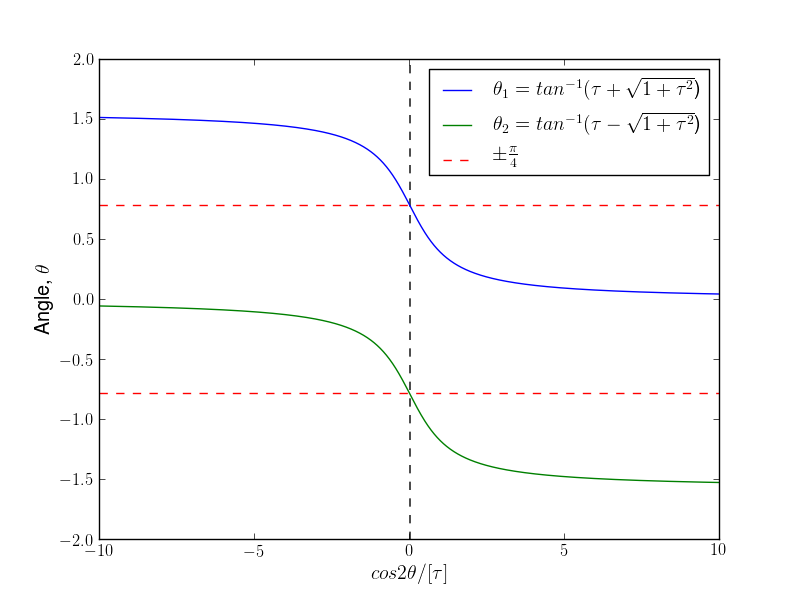
\includegraphics[scale=0.7]{fig/theta.png}
  \caption{\label{fig:theta} For hver $\tau$ får vi to muligheter for $\theta$. Fra plottet ser vi at vi alltid kan velge enten $\theta_1$ eller $\theta_2$ slik at $|\theta| \le \pi/4$ }
\end{figure}

\section{Presisjon og effektivitet}
Nå som algoritmen er implementert er det fornuftig å se på hvor godt
den fungerer. Algoritmen tar i mot et argument, $n_{\text{step}}$, som
representerer dimensjonen til matrisen i \eqref{eq:SL-matrix} vi
ønsker å bruke\footnote{Egentlig blir dimensjonen til matrisen
  $n_\text{step}-1$ når vi skal ha løsningen i $n_\text{step}+1$
  punkter. Dette kommer av grensebetingelsene som krever at løsningen
  er 0 i begge endepunktene. Disse punktene kan vi legge til i
  etterkant, og legger ikke inn ekstra tomme rader og kolonner i
  matrisen.}. Vi vet fra \eqref{eq:h-def} at en stor verdi for
$n_\text{step}$ gir en liten $h$, som generelt gir bedre nøyaktighet
for approksimasjonen vi bruker.  

Derfor ønsker vi å undersøke hvor mange punkter, $n_\text{step}$, vi
trenger for å ha nøyaktighet med, f.eks, fire ledende siffer for de
tre laveste egenverdiene. For dette har vi analytisk løsning $\lambda_0=3,\lambda_1=7,\lambda_2=11$ som vi kan bruke til å
sammenlike med. 

I tillegg til å bestemme en passende
$n_\text{step}$, må vi også sette en verdi for $\rho_\text{max}$. Vi
ser igjen fra \eqref{eq:h-def} at en større verdi av $\rho_\text{max}$
vil gi en større verdi for $h$, og dermed også mindre nøyaktighet. Men
vi må ha $\rho_\text{max}$ stor nok til at de tilhørende egenvektorene
blir med i sin helhet. 

Hvis vi begynner med å finne en passende verdi for $\rho_\text{max}$,
så skal vi foregripe begivenhetenes gang og se på figur  %veldig rar setning, hva har du ment her?
\ref{fig:three-lowest-states-non-interacting}. Figuren viser de tre
laveste energitilstandene i et system som består av to
ikke-vekselvirkende elektroner i et (3-dimensjonalt)
HO-potensial. Dersom vi kun ser på det plottet som viser løsningen for
$\omega_r=1$, er dette faktisk løsningen på en likning som er helt
ekvivalent med \eqref{eq:SL-rewrite} som vi ser på her nå. Da ser vi
at alle tre tilstandenen befinner seg innenfor $\rho\in[0,5]$. 

Noe å merke seg er at dersom vi i figur
\ref{fig:three-lowest-states-non-interacting} hadde brukt en lavere
verdi for $\rho_\text{max}$, så hadde det likevel sett ut som om
løsningene tilfeldigvis passet akkurat innenfor intervallet vi hadde
valgt. Løsningene blir ikke kappet av, men snarere trykket sammen med
høyere topper på et mindre intervall. Dette er fordi løsningene alltid
blir normaliserte slik at arealet under dem blir lik 1. Men dette
betyr ikke at løsnignene faktisk er riktige! For å se hva
$\rho_\text{max}$ faktisk må være trenger vi å velge en så stor verdi
at vi kan obervere at sannsynlighetsfordeligen faktisk dør ut
\emph{før} vi når $\rho_\text{max}$. Da kan vi heller senere
optimalisere intervallet med viten om at vi ikke ødelegger
løsningene. Et plot av typen i figur
\ref{fig:three-lowest-states-non-interacting} er en veldig fin måte å
se dette på. 

Vi ser at vi kan komme unna med forskjellige verdier for
$\rho_\text{max}$ avhengig av hvilken tilstand vi ser på. Fra figuren,
samt litt testing har vi kommet frem til noen kombinasjoner som ser
ut til å fungere nært optimalt. Med disse verdiene kan vi løse
systemet for forskjellige verdier av $n_\text{step}$ til vi finner er kombinasjon med 4 siffers
nøyaktighet. Etter litt testing\footnote{Vi brukte programmet
  \texttt{solve\_lower\_3\_states.cpp} som er tilgjengelig på Github. Programmet skriver ut egenverdiene for de tre laveste
  tilstandene.} fant vi at følge kombinasjoner ga ønsket resultat. 
\begin{itemize}
  \item[] {\makebox[2cm]{$n=0$\hfill} $\rho_\text{max} = 3.5 \cup n_\text{step}=55\rightarrow E = 2.9995$}
  \item[] {\makebox[2cm]{$n=1$\hfill} $\rho_\text{max} = 4   \cup n_\text{step}=85\rightarrow E = 6.99992$}
  \item[] {\makebox[2cm]{$n=2$\hfill} $\rho_\text{max} = 4.5 \cup n_\text{step}=90\rightarrow E = 10.9962$}
\end{itemize}

Dette er ikke \emph{veldig} store verdier for $n_\text{step}$, men
Jacobimetoden er veldig treg til å begynne med, så det tar forholdsvis
lang tid å gjøre bergningene. For å illustrere hvordan metoden ikke er
helt optimal skal vi se på hvor mange similærtransformasjoner som
brukes for å komme frem til en løsning.

Vi kan først telle opp det minimale antall transformasjoner som må
til. Siden vi her sender inn en matrise som er på tridiagonalform, og
hver transformasjon nuller ut et par med verdier, burde vi ideelt sett kunne
forvente å bruke $N-1$ transformasjoner. Vi vet imidlertidig at hver 
transformasjon også endrer elementer utenfor de tre midterste diagonalene.
Antar vi at vi trenger én transformasjon for hvert ikke-diagonale element-par(også de som begynner som 0) er det ikke
vanskelig å se at antallet transformasjoner som trengs for en $N \times N$ 
matrise er
\begin{align*}
  T(N) = (N-1) + (N-2) + (N-3) + \dots = \sum_{i=1}^{N-1}i = \frac{ 1 }{ 2 }N(N-1).
\end{align*}
En måte å se på dette er som antallet ikke-diagonale elementer
over/under diagonalen. Dette er altså det minste antallet
transformasjoner som trengs. Det faktiske antallet kaller vi $T'$.

For å se hvor mange transformasjoner metoden bruker har vi skrevet et
program som plotter $T'$ som en funksjon av $n_\text{step}$\footnote{Vi brukte programmet
  \texttt{solve\_lower\_3\_states.cpp} som er tilgjengelig på Github for
  dette.}. I samme plot er det tegnet en annengrads trendkurve for å
se tydeligere at $T'$ går som $n_\text{step}^2$. Hadde noe annet
vært tilfellet vil denne kurven ikke passet like godt. I tillegg er
det optimale antallet $T$ vi fant over tegnet i samme figur. Resultatet er vist i
figur \ref{fig:number-of-transformations}. 

Først kan vi se at trendkurven ligger på alle målepunktene vi har
laget for $T'$. Dette viser at $T'$ faktisk går som
$n_\text{step}^2$. Dette er som forventet, men det kunne hende at en
feil i implementasjonen hadde ført til å vi endte med en høyere
eksponent.

Mer interessant er det å s på forskjellen ned til den optimale
kurven. Vi ser tydelig at Jacobimetoden bruker langt flere
transformasjoner enn den strengt talt skulle trenge. Vi har faktisk at
koeffisienten forran $n_\text{step}^2$ er ca. $3.8$ ganger større for
$T'$ sammenliknet med $T$. 

Alle de ekstra transformasjonene kommer fra at når vi utfører en
similærtransformasjon for å nulle ut et par med matriseelementer, er
det en sjanse for at et annet element vi allerede har nullet ut
faktisk blir ikke-null. Da må vi gå tilbake å gjenta prosessen flere
ganger for samme element, og dette ender med effekten vist i figur \ref{fig:number-of-transformations}.

\begin{figure}[ht]
  \centering
  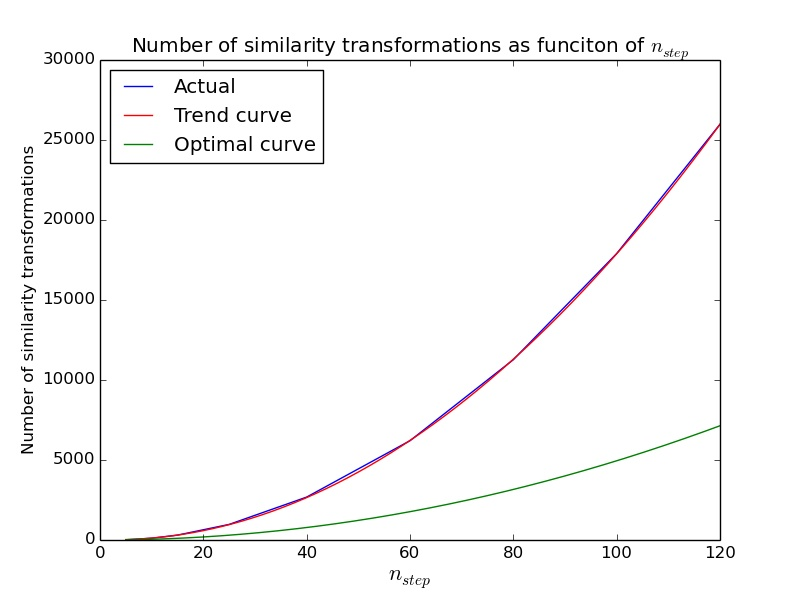
\includegraphics[scale=0.5]{fig/number_of_transformations_trend_plot.jpg}
  \caption{\label{fig:number-of-transformations} Plott av antall
    similærtransformasjoner Jacobimetoden bruker som en funksjon av
    dimensjonen til matrisen som transformeres. En annengrads
    trendkurve er tegnet på og viser at antallet passer godt med en
    annengradfunksjon. Det minimale antallet også tegnet opp, og vi
    ser hvor mye ekstra metoden bruker. Koeffisienten forran
    $n_\text{step}^2$ er omtrent $3.8$ ganger større enn for den
    optimale kurven.}
\end{figure}

\begin{figure}[ht]
  \centering
  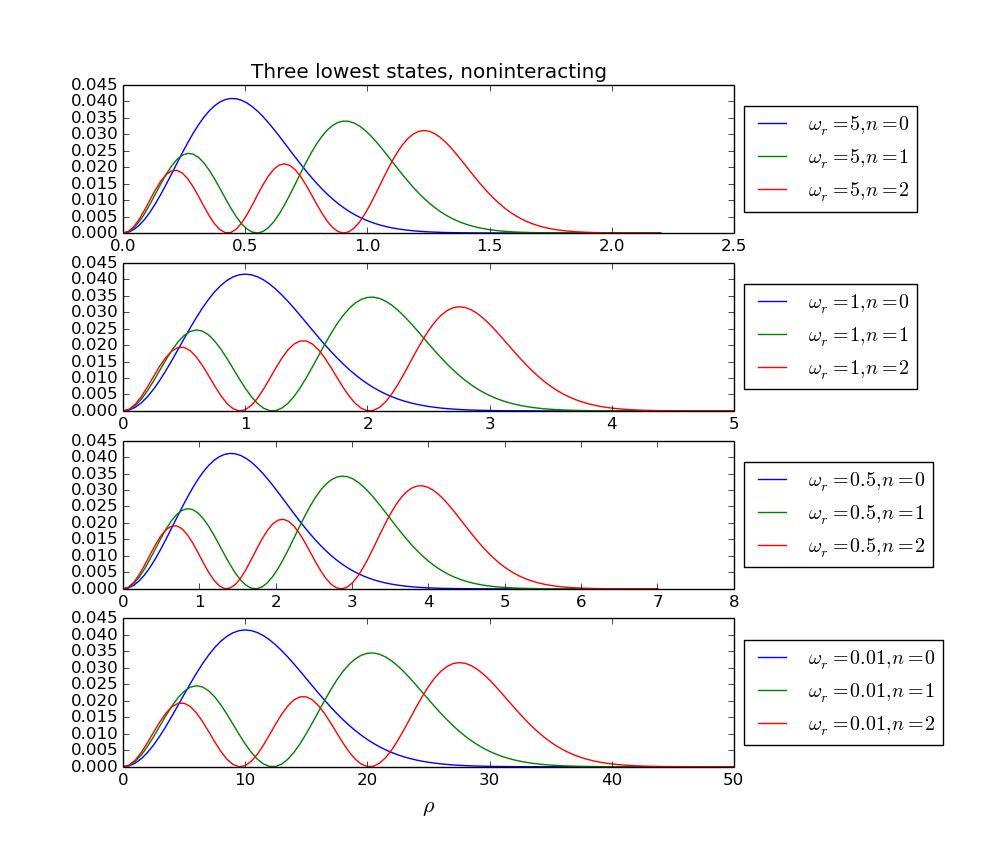
\includegraphics[scale=0.65]{fig/three_lowest_states_noninteracting.png}
  \caption{\label{fig:three-lowest-states-non-interacting} Figuren viser
    de tre laveste energitilstandene i det tilfellet der de to
    elektronene ikke vekselvirker. Hvert plot viser hvordan formen ser ut
    for ulike verdier av $\omega_r$. Merk også forskjellen på
    intervallet til $\rho$ i de forskjellige tilfellene. Alle
    løsningene er for tilfellet der $l=0$.}
\end{figure}

\begin{figure}[ht]
  \centering
  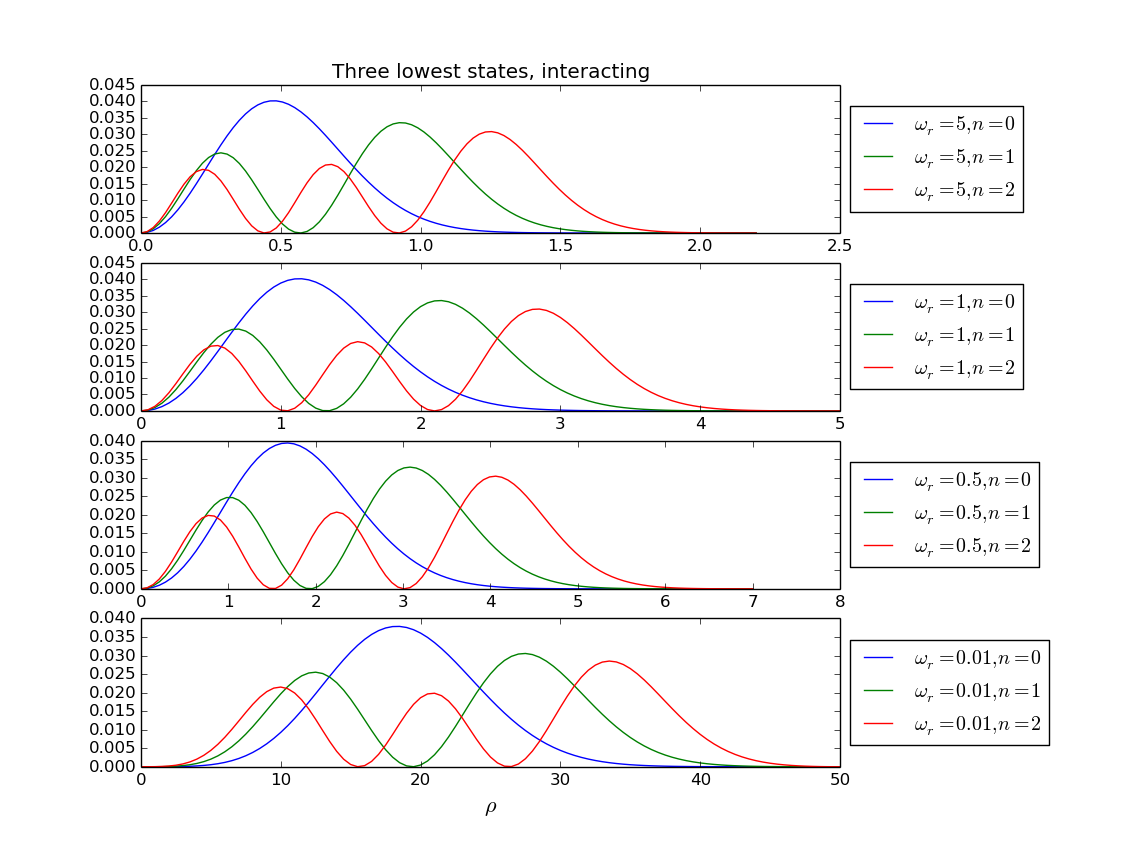
\includegraphics[scale=0.65]{fig/three_lowest_states_interacting.png}
  \caption{\label{fig:three-lowest-states-interacting} Figuren viser
    de tre laveste energitilstandene i det tilfellet der de to
    elektronene vekselvirker. Hvert plot viser hvordan formen ser ut
    for ulike verdier av $\omega_r$. Merk også forskjellen på
    intervallet til $\rho$ i de forskjellige tilfellene. Alle
    løsningene er for tilfellet der $l=0$.}
\end{figure}

\printbibliography
\end{document}
%%% Local Variables:
%%% mode: latex
%%% TeX-master: t
%%% End:
